\section{Caches}

\subsection{Caches de premier niveau L1}

Au cours précédent, nous avons étudié le comportement d'un automate pré-programmé
qui effectuait machinalement des tâches d'opérations et de requêtes à un ou plusieurs
composants cibles.\\Néanmoins, dans le cas d'un automate reprogrammable comme le
MIPS32, utilise des intermédiaires pour ses accès mémoires en l'objets de caches.
Plus spécifiquement de contrôleurs de caches, afin d'éviter une temporisation du
processeur.

\subsection{Principes des mémoire caches}

La performance des caches est basée sur deux principes intrinsèques à la nature
des données en mémoire :

\begin{itemize}
  \item La localité spatiale, soit deux adresses X et X', après lecture de X,
  plus X' est proche de X, plus sa probabilité d'être la prochaine adresse
  requise est élevée. La localité spatiale a pour critère principale la
  contiguité des données.\\
  Ex: lecture d'nu tableau, lecture (souvent [tojours]) séquentielle des
  instructions.
  \item La localité temporelle, soit une adresse X, après lecture de X, plus de
  temps s'écoule entre cet accès et le prochain, et plus sa probabilité d'être
  encore la prochaine adresse requise est basse. La localité temporelle a pour
  critère principale la réutilisabilité des données.\\
  Ex: exécution d'une boucle d'instruction
\end{itemize}
  \begin{center}
    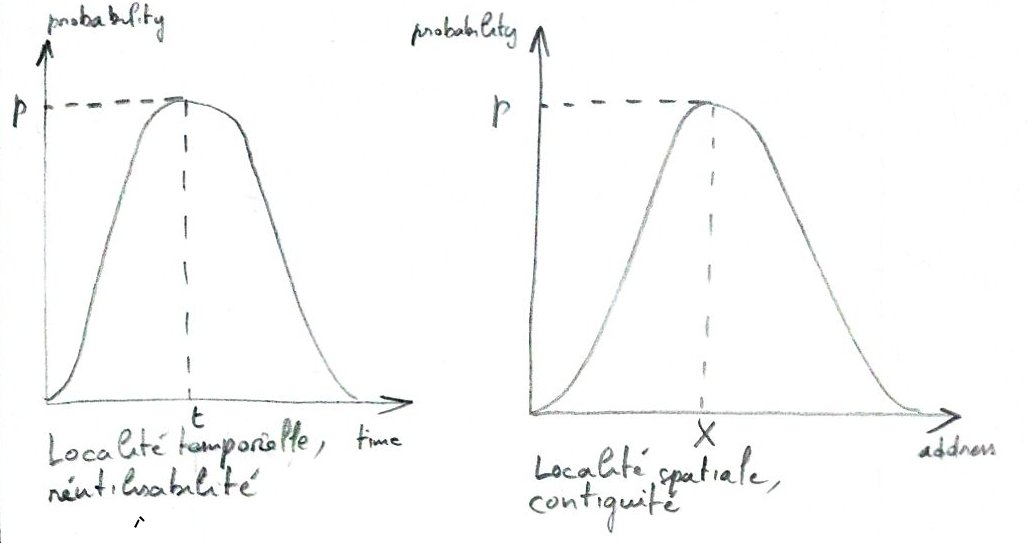
\includegraphics[width=11cm]{cours3/pics/charts.jpg}
  \end{center}

\subsection{Vocabulaire}

\begin{itemize}
  \item {\bf Alignement} : une portion de la mémoire est dite alignée si et
  seulement si son adresse de base est multiple de la longeur de la portion.

  \item {\bf Ligne de cache} :\\
  nombre fixe d'octets à des adresses consécutives et alignées (multiples de 4).
  Elle représente une portion de l'espace adressable.\\
  Sur une architecture MIPS32 l'espace adressable est partitioné en
  $\frac{2^{32}}{2^4}={2}^{28}={2}^{10}\times{2}^{10}\times{2}^{8}=256$ million
  de lignes.\\
  Nous considérerons des lignes de caches de 16 octets : \\
  \begin{center}
    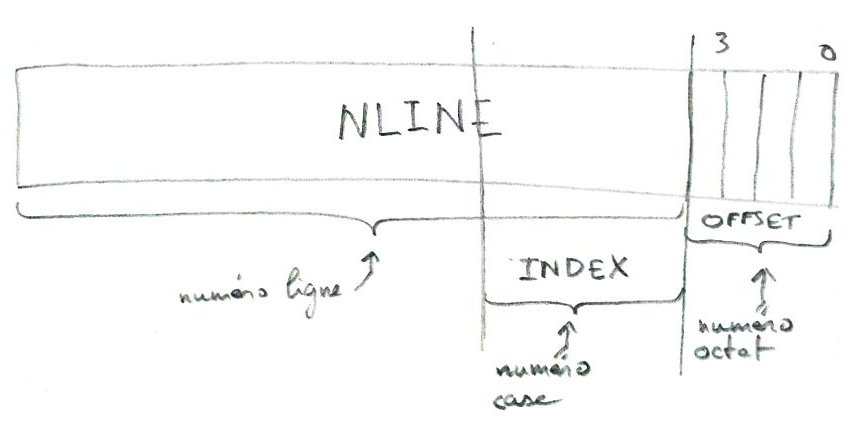
\includegraphics[width=11cm]{cours3/pics/adress.jpg}
  \end{center}
  \item {\bf Cache à Correspondance Directe} :\\
  Une ligne de cache ne peut avoir qu'une case prédéfinie dans la mémoire cache.

  \item {\bf Cache Associatif} :\\
  \begin{itemize}
    \item {\it Associatif Complet} :\\
    Toute ligne du cache peut être stockée dans n'importe quelle case dans la
    mémoire cache.
    \item {\it Associatif par Ensemble} :\\
    Une ligne de cache peut avoir un certain nombre de cases prédéfinies dans la
    mémoire cache, selon le degré d'association.
  \end{itemize}

  \item {\bf Politique Write-Through} :\\
  Toute requête d'écriture du procésseur est envoyée à la mémoire, sans attente,
  sur le bus. Le Tampon d'Écritures Postées permet au processeur de ne pas être
  bloqué sous réserve de tampon non-plein.

  \item {\bf Politique Write-Back} :\\
  Toute écriture d'une adressse X de la part du processeur est effectuée dans le
  cache L1. S'il y a MISS, alors le processeur requiert que la ligne conenant X
  soit ramenée dans le cache.

  \item {\bf Tampon d'Écriture Postée} :\\
  Le TEP est un composant permettant de mettre en attente plusieurs requêtes vers
  le PIBUS sans pour autant geler le processeur (sous réserve du tampon non-plein).\\
  Un mécanisme d'implémentation parmi d'autres du TEP est le protocole FIFO.
\end{itemize}

\subsection{Spécifications du cache L1 vu en cours}
\begin{itemize}
  \item 2 caches séparés pour instructions et données :\\
  Cela permet un comportement pipeline, avec les émissions de requètes de lectures
  d'instructions et d'accès mémoire possible
  \item Politique Write-Through : \\
  simplifie les problèmes de cohérence
  \item Associatif par ensemble paramètrable :
  \begin{itemize}
    \item NWORDS : nombre de mots par lignes
    \item NSETS : nombre d'ensembles
    \item NWAYS : degré d'associativité (NWAYS = 1 $Rightarrow$ Correspondance
    Directe).
    \item ${NWAYS}\times{NSETS}\times{NWORDS}={\#Cache}$
  \end{itemize}
  \item {\bf Bloquant} :\\
  Tant que le cache n'a pas aquitté de la requête du processeur, ce dernier est
  bloqué (parce que le MIPS32 est pipeline scalaire, ce n'est pas le cas pour les
  processeurs superscalaires par exemple).
\end{itemize}

\subsection{Spécifications des Interfaces 1}
\begin{center}
  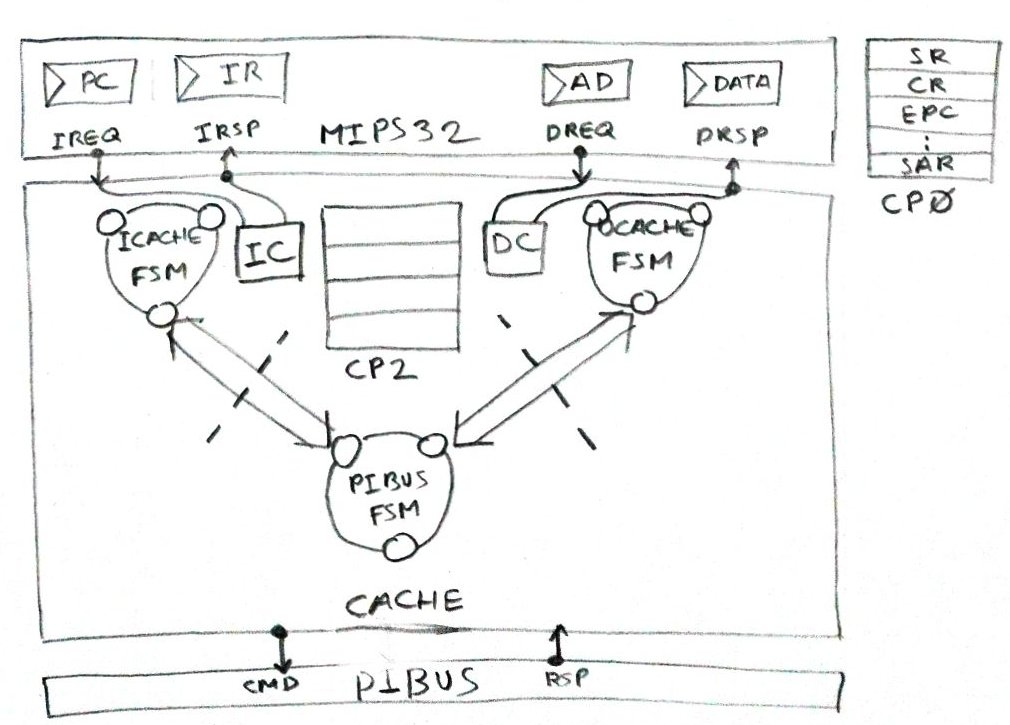
\includegraphics[width=17cm]{cours3/pics/cache_internal.jpg}
\end{center}
\begin{itemize}
  \item {\bf IREQ} :\\
  \begin{itemize}
    \item addr(30) : 30 bits de poids forts car alignée (multiple de 4)
    \item valid(1) : envoi ou non de la requête
    \item mode(1) : utilisateur ou système
  \end{itemize}
  \item {\bf IRSP} :\\
  \begin{itemize}
    \item instr(32)
    \item valid(1) : bloque le processeur si égal à 0
    \item error(1) : prévient d'une erreur de bus si égal à 1
  \end{itemize}
  \item {\bf DREQ} :\\
  \begin{itemize}
    \item addr(30) : 30 bits de poids forts car alignée (multiple de 4)
    \item valid(1)
    \item mode(1)
    \item type(3) : voir spécification du signal DTYPE
    \item wdata(32)
    \item byte\_enable : spécifie les octets à écrire (codage one-hot)
  \end{itemize}
  \item {\bf DRSP} :\\
  \begin{itemize}
    \item rdata(32)
    \item valid(1)
    \item error(1)
  \end{itemize}
  \item {\bf DYTPE} :\\
  \begin{itemize}
    \item READ
    \item Write
    \item Linked\_Load
    \item Store\_Cond\\
    Opérations pour implémenter l'accès atomique à une ressource
    \item XTN\_READ
    \item XTN\_WRITE\\
    Accès en dehors de l'espace adressable courant (ex : co-processeurs)
  \end{itemize}
\end{itemize}
